\chapter{Introduction}

\section{CERN}

The European Organization for Nuclear Research, or CERN, is an institution tasked with providing particle accelerators to scientists for purposes of conducting high energy physics experiments. It is the home of the Large Hadron Collider (LHC) accelerator complex, comprised primarily of LINAC4, the Proton Synchrotron (PS), Proton Synchrotron Booster (PSB), Super Proton Synchrotron (SPS) and the Large Hadron Collider (LHC). It is located across the Franco-Swiss border local to Lake Geneva, the Jura mountains, and Mont Salève.

\begin{figure}
    \centering
    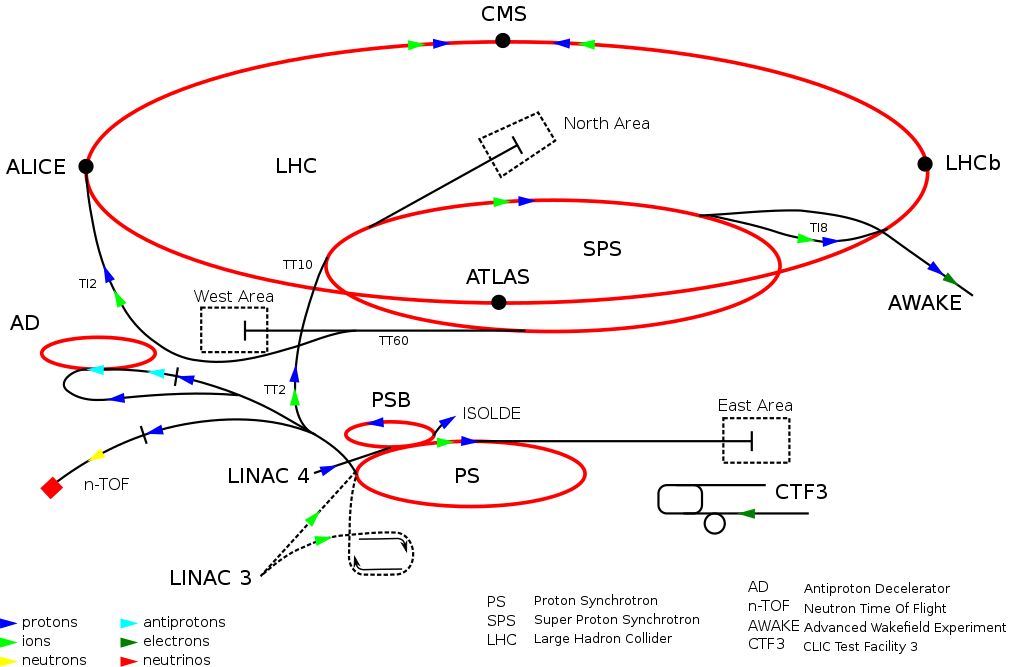
\includegraphics{figs/1024px-Cern-accelerator-complex.svg.png}
    \caption{The CERN Accelerator Complex}
    \label{fig:cern}
\end{figure}

The particle's produced in proton-proton collisions by the LHC can vary in charge, spin, mass, momentum, etc. and accordingly the qualities of these decay products must be quantified through the use of large particle detector systems. Typically they are comprised of solenoids to probe the particle's momentum via magnetic rigidity, calorimeters to estimate particle energy deposition, and micro-channel plates to probe time-of-flight and generalized tracking as depicted in Figure \ref{fig:cms}.

\begin{figure}
    \centering
    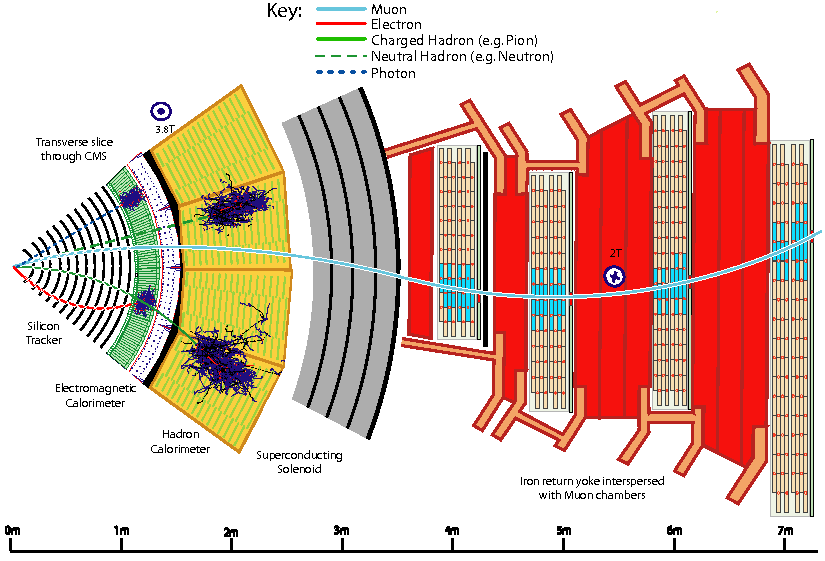
\includegraphics{figs/cms_detector.jpg}
    \caption{Radial evolution of particles through CMS detector, generated by collisions within the LHC}
    \label{fig:cms}
\end{figure}

In the case of the Compact Muon Solenoid (CMS) detector, Figure \ref{fig:cms}, proton-proton collisions emit muons, electrons, hadrons and photons which  subsequently influence the detector subsystems and trackers. Due to statistical variation of the beam collision and variability of particle interactions observed, trajectories need to be studied and analyzed over long periods of time to provide the best statistical utility for physics.

\begin{figure}
    \centering
    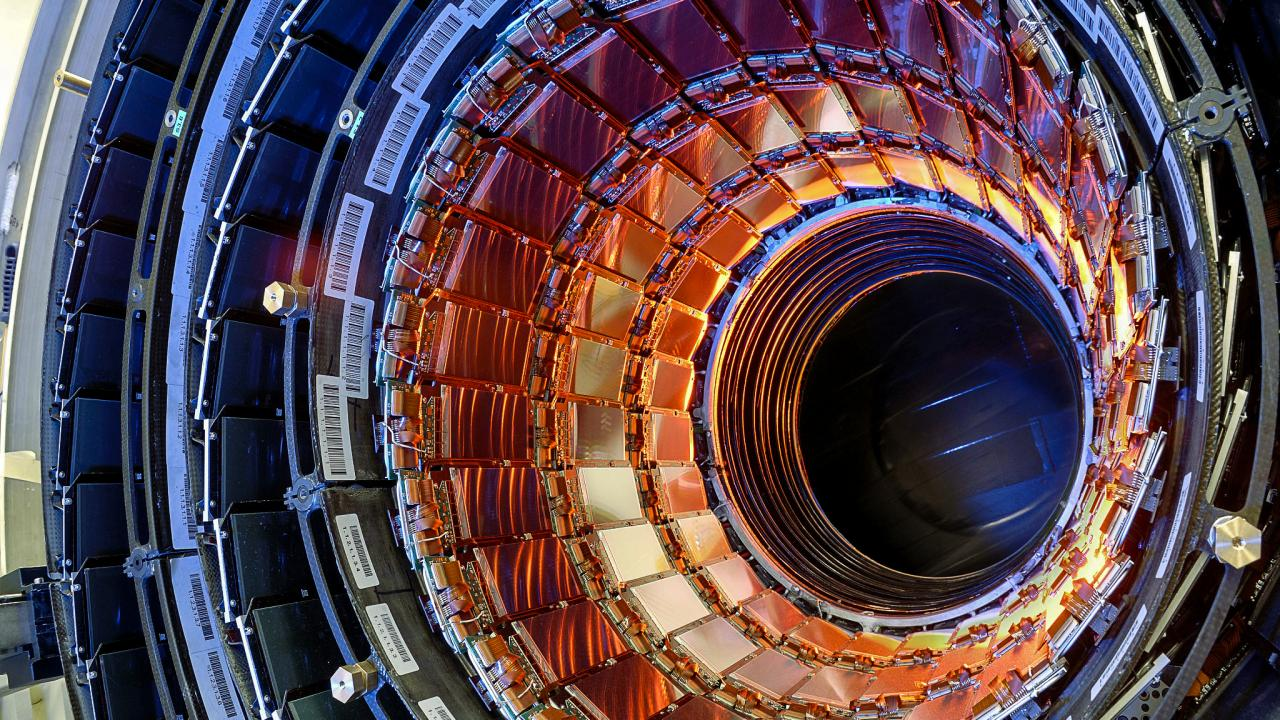
\includegraphics{figs/sn-LHC.jpg}
    \caption{Internals of CERN's CMS Muon Detector}
    \label{fig:cms_internals}
\end{figure}

The quality of data is correlated with the overall exposure of the detectors to collision events and so accordingly the uncertainty of certain measurements can be improved by increasing the total integrated exposure time, and by increasing the total beam quality or luminosity ($\mathcal{L}$), so that the events of interest are occurring in greater number. We see in Equation \ref{eq:luminosity} how for a bivariate gaussian beam, the luminosity scales with number of bunches $n_B$, particles per bunch $N$ and inversely width beam width $\sigma$. Accordingly, there is an ever persistent engineering effort to improve the beam luminosity throughout the CERN accelerator chain, typically by increasing factors such as beam intensity, reducing bunch emittance, beam size and divergence, improve stability and variation, etc.

\begin{equation}
    \mathcal{L} = \frac{n_bN^2f_{rep}}{4\pi\sigma_x\sigma_y}H_d
    \label{eq:luminosity}
\end{equation}

As particle beam's intensities are increased to increase luminosity, the self electromagnetic fields of the charged particles within a bunch will begin to have an effect on the bunch itself. This self interaction is name \textit{space-charge}, the phenomena where the very composition of a bunch can cause the bunch itself to repel apart, break up or induce other instabilities and perturbations. These instabilities typically have a negative impact on the usefulness of the beam towards scientific applications and accordingly space-charge instabilities and other effects need to be effectively characterized, suppressed or otherwise mitigated.

\section{The Proton Synchrotron}

Space-charge effects typically reduce with particle energy and so for higher energy accelerators, or rings with minimal bunch intensity, space-charge can be often overlooked. CERN's Proton Synchrotron (PS) however is a rather unique device in that through it's particle ramp cycle, the bunch transitions between regimes where space-charge is initially dominated to regimes where it can be effectively ignored. It is also a device which experiences the phenomena of "transition crossing", an dynamic period during the life of a particle bunch where the stability bucket jumps drastically and proactive measures must be taken to retain bunch stability

\begin{figure}
    \centering
    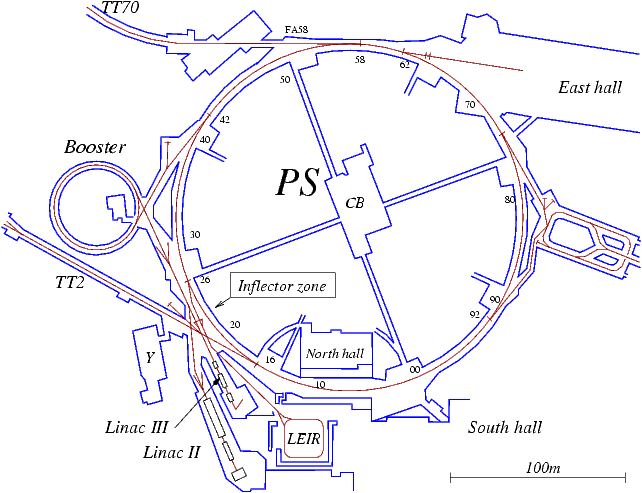
\includegraphics{figs/pscomplex.png}
    \caption{The PS complex}
    \label{fig:ps_complex}
\end{figure}

Parameter's summarizing injection and extraction characteristics at flat-bottom and flat-top respectively are represented in Table \ref{tab:ps_parameters}.

\begin{table}
    \centering
    \begin{tabular}{lccc}
        Parameter                  & Symbol        & Injection                      & Extraction \\
        \hline
        Circumference (m)          & C             & \multicolumn{2}{c}{628}                     \\
        Kinetic Energy (GeV)       & W             & 1.4                            & 25         \\
        Lorentz Factor             & $\gamma$      & 2.5                            & 27.7       \\
        Revolution Frequency (kHz) & $f_s$         & 436                            & 476        \\
        RF Harmonic                & $h$           & 7                              & 21         \\
        RF Frequency (MHz)         & $f_{RF}$      & 3                              & 10         \\
        Synchrotron Frequency (Hz) & $\Omega_s$    & 600                            & 230        \\
        Synchrotron Tune           & $Q_s$         & 0.00137                        & 0.00048    \\
        Transverse Tune            & $Q_x, Q_y$    & \multicolumn{2}{c}{6.21, 6.24}              \\
        Transition Factor          & $\gamma_t$    & 6.1                            & 6.1        \\
        Bunch Width (ns)           & $\sigma_\tau$ & 26                             & 1
    \end{tabular}
    \caption{Injection/Extraction parameters for PS at flat-top"' and 'flat-bottom' respectively.}
    \label{tab:ps_parameters}
\end{table}

The PS provides an opportunity to perform experiments with highly intense proton beams over a large energy range relevant for space charge studies. In standard operation, the configuration of RF profile ramp parameters for an LHC run is represented in Figure \ref{fig:ps_ramp}. PS particle bunches are typically comprised of 8e+12 particles \cite{migliorati_instability_2018}, highly intense for only mildly relativistic energies.

\begin{figure}
    \centering
    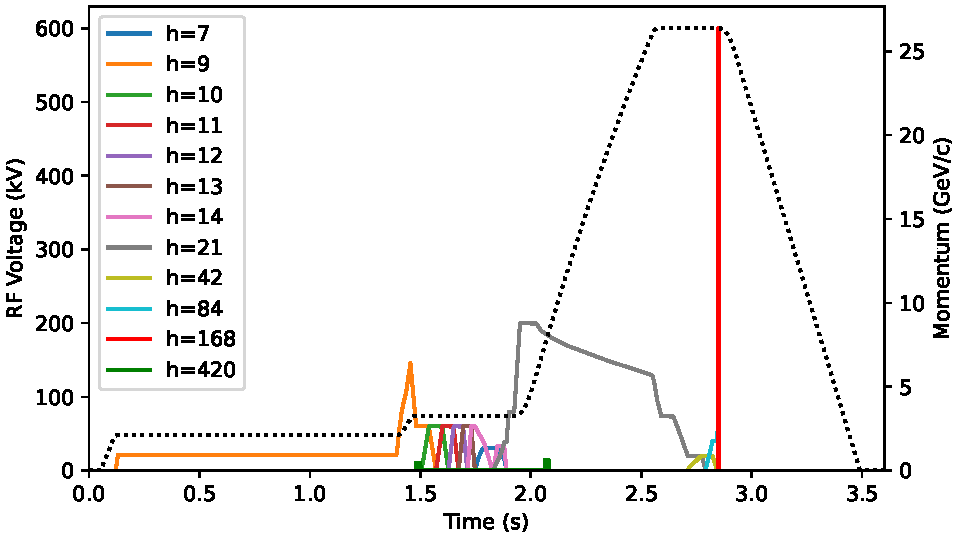
\includegraphics{figs/ps_profiles.pdf}
    \caption{RF harmonic ramp profiles for PS}
    \label{fig:ps_ramp}
\end{figure}

\section{Motivation}

As will be discussed further, the stability of our bunch occupies two regimes, first the space-charge dominated regime and later the regime dominated by inductive impedance. Depending on the bunch intensity and bunch length properties, these regimes produce focusing/defocusing effects surrounding transition and are observed to compensate for one another near transition.

\subsection{Space-Charge Impedance Compensation}

The space-charge impedance of the PS during its ramp cycle is given in Figure \ref{fig:ps_impedance}. It shows that the effective longitudinal impedance due to space-charge is approximately compensated by the PS's inductive impedance near transition energies. This therefore defines this regime as highly dynamic and of particular interest for space-charge studies in the PS.

\begin{figure}
    \centering
    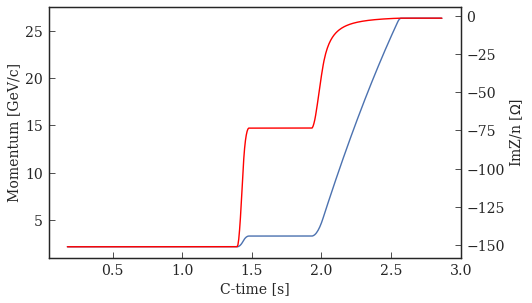
\includegraphics{figs/energy_v_space_charge_impedance.png}
    \caption{Proton \textcolor{blue}{momentum} vs. \textcolor{red}{inductive impedance} during PS Ramp}
    \label{fig:ps_impedance}
\end{figure}

\subsection{Validation of Longitudinal Space-Charge Trackers}

When current space-charge approximations are incorporated into longitudinal tracking codes such as \href{https://blond.web.cern.ch/}{BLonD} \cite{noauthor_cern_nodate}, we can observe that the bunch length oscillations amplitude and frequency can only be matched when current space-charge calculations are reduced by roughly 30\%, as seen in Figure \ref{fig:BlonD_v_experiment}. This discrepancy may suggest that there may exist an additional stabilizing phenomena within which the current model for longitudinal space-charge impedance is neglecting.

\begin{figure}
    \centering
    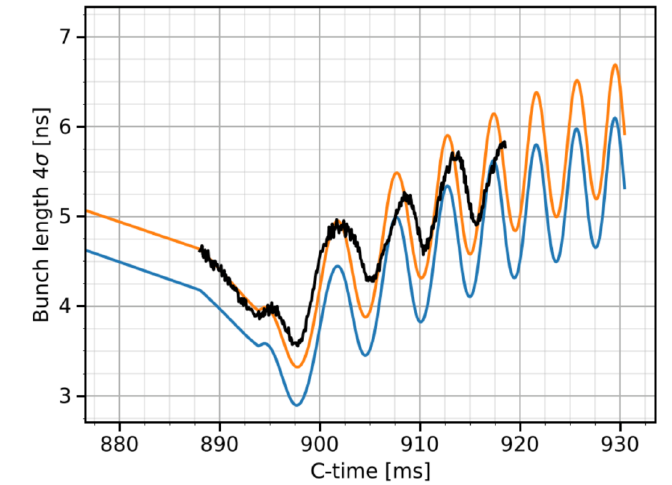
\includegraphics{figs/simulation_v_experiment.png}
    \caption{Bunch length oscillation simulation benchmarked with experiment}
    \label{fig:BlonD_v_experiment}
\end{figure}

A possible candidate to describe this discrepancy may be related to the fact that current longitudinal codes neglect transverse betatron motion, suggesting that the variance in individual transverse particle trajectories may lead to describing new phenomena in the longitudinal plane.

\subsection{Micro-Bunch Instabilities}

Because there is a causal relationship with how space-charge wakefields fields emitted from the front of a bunch propagate toward the tails, small perturbations and density fluctuations in the bunch's longitudinal charge density profile can create local fluctuations that can self-amplify leading to \textit{micro-bunch instabilities}. This phenomena becomes a challenge for very intense and short bunches that can rapidly destabilize an otherwise well behaved distribution.

\begin{figure}
    \centering
    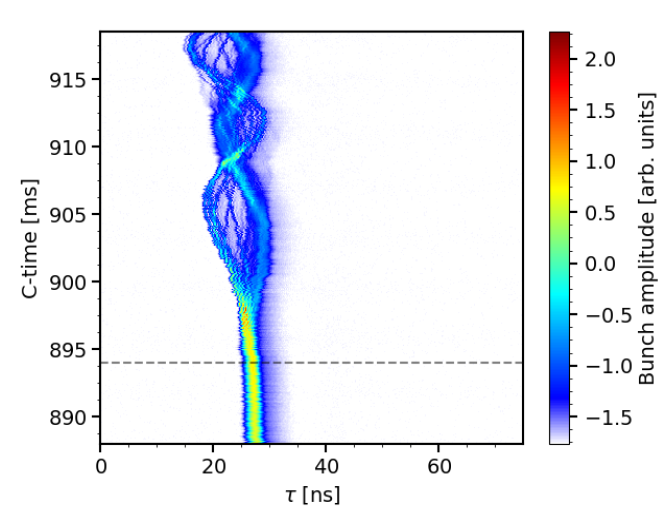
\includegraphics{figs/micro_bunching_instabilities.PNG}
    \caption{Example of micro-bunch instabilities simulated in a Longitudinal Tracking Code}
    \label{fig:microbunch_instabilities}
\end{figure}

As seen in Figure \ref{fig:microbunch_instabilities}, a narrow bunch distribution can spontaneously split due to local fluctuations in the bunch profile that have a negative feedback mechanism for promoting further instabilities. With time, the bunch will "filament" and the longitudinal fluctuations will smoothen out but at a cost in total beam quality.

\chapter{Beam Dynamics}

\section{Transverse Dynamics}

\subsection{Betatron Motion}

A particle's transverse position $u(s)$ and divergence $u'(s)$ within a focusing lattice characterized by the beta function $\beta(s)$, is dependent on particle emittance $\epsilon$ and phase $\phi$:

\begin{equation}
    u(s)=\sqrt{\beta\epsilon}\cos\phi \qquad u'(s)=-\sqrt{\frac{\epsilon}{\beta}}(\alpha\cos\phi+\sin\phi)
    \label{eq:hills_equations}
\end{equation}

The phase advance $\mu(s)$ from a particle's initial phase offset $\mu_0$ is given by:

$$\phi = \mu(s) + \mu_0 \qquad \mu(s) = \int_0^s\frac{ds}{\beta(s)}$$

Accordingly, betatron motion follows elliptical $u$-$u'$ trajectories per a particle's emittance $\epsilon$ and it's Twiss parameters $\alpha$, $\beta$ and $\gamma$ \cite{courant_theory_1958}.

$$\epsilon = \gamma u^2 + 2 \alpha u u' + \beta u'^2$$

Where from a continuous beta function $\beta(s)$, the Twiss parameters can be derived:

$$\alpha(s) = -\frac{1}{2}\beta'(s) \qquad \gamma(s) = \frac{1+\alpha(s)^2}{\beta(s)}$$

We can incorporate particle dispersion $\delta$ when also provided with the dispersion function $D(s)$:

$$u(s) = u_\beta + u_D= \sqrt{\beta\epsilon}\cos\phi + D\delta$$

A bivariate transverse distribution ($x$-$x'$, $y$-$y'$) can be statistically described by its covariance matrix $\Sigma$, the product of its ``root-mean-square" emittance $\epsilon$ and the Twiss matrix $\Omega$, encapsulating the focusing properties of the present optics.

$$\Sigma = \begin{bmatrix}<x^2> & <xx'> \\ <x'x>& <x'^2>\end{bmatrix} = \epsilon\Omega \qquad \Omega = \begin{bmatrix}\beta &-\alpha \\ -\alpha & \gamma\end{bmatrix} \qquad \epsilon = \sqrt{\det(\Sigma)}$$

Such that an injected particle distribution's covariance matrix matches that of the optics $\Omega$, the collective motion of the bunch will be such that the beam width throughout the ring can be described by:

$$\begin{aligned}
        \sigma^2_x(s) & = \beta_x(s)\epsilon_x+D(s)^2\sigma_\delta^2 \\
        \sigma^2_y(s) & = \beta_y(s)\epsilon_y
    \end{aligned}$$

As consistent in Figure \ref{fig:ps_transverse_tracking}, individual particle trajectories are seen in faded chaotic paths whereas the bulk group motion of the bunch width is seen to be defined by the "strong focusing" of the optics for a matched distribution.

\begin{figure}
    \centering
    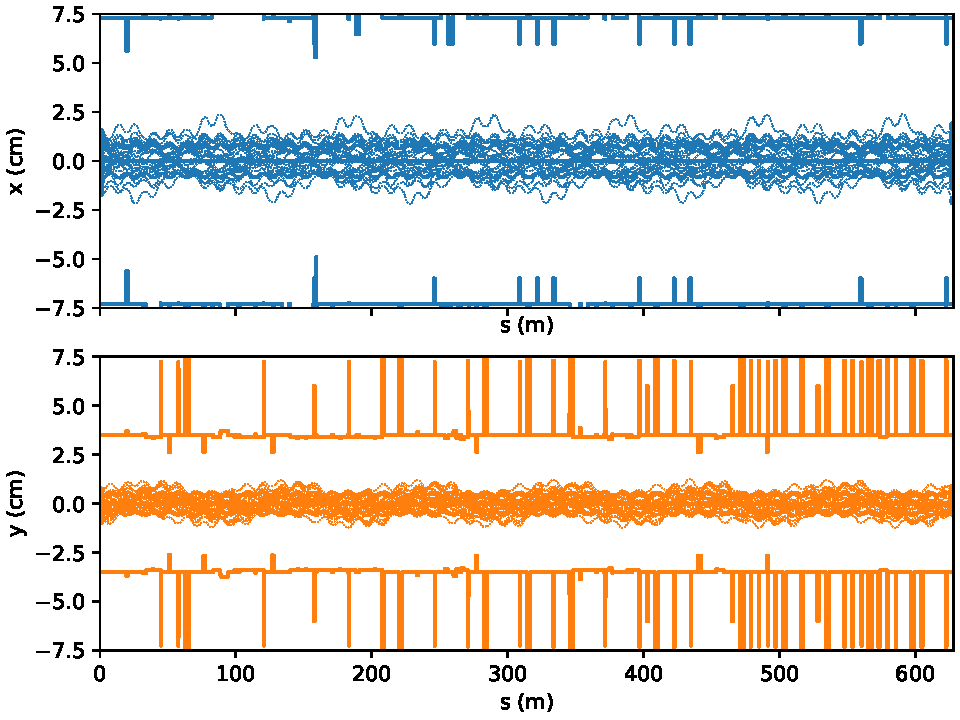
\includegraphics{figs/ps_aperture.multivariate.pdf}
    \caption{Strong focusing of betatron motion matched to PS Optics}
    \label{fig:ps_transverse_tracking}
\end{figure}

\section{Longitudinal Motion}

\subsection{Single Particle Motion}

\subsubsection{Energy Kick}

In longitudinal motion, our phase-space can be defined by time-momentum ($t$, $p$) or phase-energy ($\varphi$, $W$) coordinates. In phase-space relative to the synchronous particle (indicated by subscripted s) our coordinates are defined as follows:

$$\tau = t - t_s \qquad \delta = \frac{p-p_s}{p_s} \qquad \phi = \varphi - \varphi_s \qquad w = W-W_s$$

The energy gain of a particle accelerated through an RF gap along a turn can given by $\Delta W=qV_g\sin\varphi$ \cite{panofsky_considerations_1956} where in relative coordinates we have:

$$\Delta w = q V_g(\sin\varphi-\sin\varphi_s)=q V(\tau)$$

The effective gap voltage is given by $V(\tau) = V_g g(\phi)$ with gap voltage $V_g$ and relative phase given by $\phi = h\omega_s\tau$, the RF field gradient is given by $g(\phi)=\sin(\phi+\varphi_s)-\sin\varphi_s$ so that $g'(\phi)=\cos(\varphi_s-\phi)$ and $G(\phi)=(1-\cos\phi)\cos\varphi_s+(\sin\phi-\phi)\sin\varphi_s$.

\subsubsection{Particle Drift}

In a drift a particles revolution period $T$ evolves with energy $E$ given by:

$$\frac{dT}{T} = \frac{\eta}{\beta^2}\frac{dE}{E} \qquad \eta =\alpha- \frac{1}{\gamma^2} \qquad \alpha = \frac{dC/C}{dp/p} = \frac{1}{\gamma_t^2}$$

Where our slippage factor $\eta$ is given by the momentum compaction factor $\alpha$ and the particle's Lorentz factor $\gamma$ defined by it's transition energy $\gamma_t$.

For convenience, we define:

$$\kappa = \frac{\eta}{\beta_s^2E_s} $$

Combined, a particle's evolution in phase-space can be described as the combination of a voltage "kick" and a phase "drift" each turn around the ring. Accordingly, the equations of motion can be given as follows:

\begin{equation}
    \dot{\tau} = \kappa w \qquad \dot{w} = \frac{qV(\tau)}{T_s}
    \label{eq:eom}
\end{equation}

For a linear applied voltage $V(\tau) \approx V'(\tau)\tau$, we can derive a phase equation as simple harmonic motion with oscillation frequency $\Omega$ by:

$$\ddot{\tau}+\Omega^2\tau = 0 \qquad \Omega^2 = -\frac{\kappa q}{T_s}V'(\tau)$$

Therefore we can identify that the amplitude of our synchrotron oscillation frequency broadly varies as the square of the effective voltage gradient:

$$\Omega \propto \sqrt{V'(\tau)}$$

For small-amplitude oscillations where $\phi \to 0$, $g'(\phi) \approx \cos\varphi_s$ and so $V'(\tau)\approx h\omega_s V_g \cos\varphi_s$. This yields the canonical definition for the \textit{Synchrotron Frequency}. 

\begin{equation}
    \Omega_s^2 = -\frac{h\omega_s^2\eta}{\beta_s^2\gamma_s}\frac{qV_g}{2\pi}\cos\varphi_s
    \label{eq:synchrotron_frequency}
\end{equation}

\subsection{Hamiltonian}

Our equations of motion can be derived from the following Hamiltonian:

$$\begin{aligned}
        H & = \frac{1}{2}\kappa w^2 -\frac{q}{T_s}\int V(\tau)d\tau \\
          & = \frac{1}{2}\kappa w^2 -\frac{q V_g}{2\pi h}G(\phi)
    \end{aligned}$$

such that Hamilton's equations are obeyed:

$$\frac{dH}{dw} = \dot{\tau} \qquad -\frac{dH}{d\tau} = \dot{w}$$

We can then re-write our trajectories as a function of the particles conserved hamiltonian value as functions of maximum oscillation amplitudes $\hat{\tau}$ and $\hat{w}$.

$$H = -\frac{qV_g}{2\pi h}G(\hat{\phi}) = \frac{1}{2}\kappa \hat{w}^2$$

$$w(\tau) = \pm \sqrt{\frac{2}{\kappa}\left(H+\frac{q}{T_s}\int V(\tau) d\tau\right)}$$

Given that $\dot{\phi} = h\omega_s\dot{\tau}$ and $W(\phi) = G(\phi)/\cos\varphi_s$, we can define our particle trajectories arbitrarily by:

$$\dot{\phi} = \Omega_s\sqrt{2(W(\hat{\phi})-W(\phi))}$$

We can see these trajectories visualized in Figure \ref{fig:fisheye}. Particles oscillating near the center with small oscillation amplitudes $\hat{\tau}$ retain elliptical trajectories whereas particles with larger values in $\hat{\tau}$ experience non-linear and asymmetric RF forces, yielding a ``fish" shape.

\begin{figure}
    \centering
    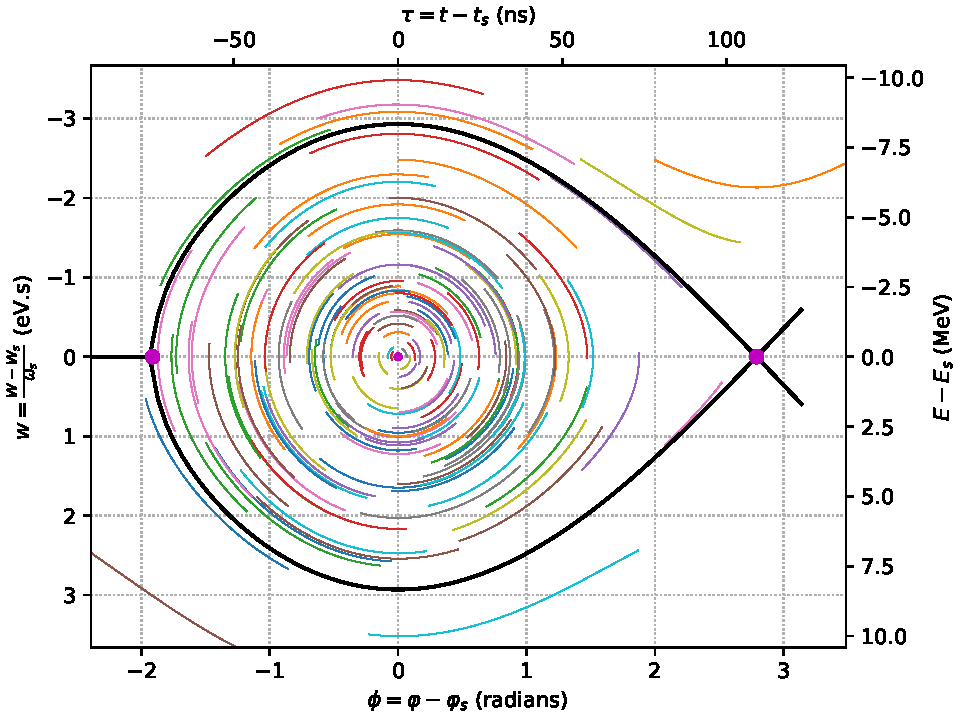
\includegraphics{figs/single_particle_motion/trajectories.pdf}
    \caption{Particle trajectories circulating along Hamiltonian contours}
    \label{fig:fisheye}
\end{figure}

The separatrix (in black) defines the contour of the hamiltonian's local maximum such that within, particles will retain stable trajectories. Particles injected outside the separatrix will follow unstable trajectories.

\subsection{Tune Spread}

The synchrotron period  ($\Pi$) of a particle with given oscillation amplitude $\hat{\phi}$ between the left $\phi_L$ and right $\phi_R$ limits is computed by:

$$\Pi = \oint \frac{d\phi}{\dot{\phi}} = \frac{2}{\Omega_s}\int_{\phi_L}^{\phi_R} \frac{d\phi}{\sqrt{2(W(\hat{\phi})-W(\phi))}}$$

For a \textit{non-accelerating bucket}, $\varphi_s = 0$. Therefore $G(\phi) \to \cos\varphi_s(1-\cos\phi)$, $\phi_R = \hat{\phi}$ and $\phi_L = -\hat{\phi}$ resulting in:

$$\Pi = \frac{4}{\Omega_s\sqrt{2}}\int_0^{\hat{\phi}}\frac{d\phi}{\sqrt{\cos\phi-\cos\hat{\phi}}} = \frac{4K(\hat{\phi}/2; k=\csc(\hat{\phi}/2))}{\Omega_s}$$

Defining the normalized synchrotron tune $\mu$ via $\mu = \Omega(\hat{\phi})/\Omega_s$ yields:

\begin{equation}
    \mu =\frac{\pi}{2K(\frac{\hat{\phi}}{2})} \approx 1-\frac{\hat{\phi}^2}{16} \qquad \phi \approx 4\sqrt{1-\mu}
    \label{eq:tune_spread}
\end{equation}

Accordingly, a distribution of linear charge density $\lambda(\phi)$ corresponds to a spread in normalized synchrotron tune $\mu$.

\begin{table}
    \centering
    \begin{tabular}{c|c|c|c}
                  & $\lambda(\phi)$                                                                                                   & $\lambda(\mu)$                                                                              & $d\lambda/d\phi$                      \\
        \hline
        Gaussian  & $\frac{1}{\sigma_{\hat{\phi}}\sqrt{2\pi}}\exp\left(-\frac{1}{2}\frac{\hat{\phi}^2}{\sigma_{\hat{\phi}}^2}\right)$ & $\frac{1}{\sigma_{\hat{\phi}}\sqrt{2\pi}}\exp(-\frac{1}{2}\frac{16(1-\mu)}{\sigma_\phi^2})$ & $-\frac{\phi}{\sigma^2}\lambda(\phi)$ \\
        Parabolic & $\frac{3}{2L_{\hat{\phi}}}(1-4\frac{\hat{\phi}^2}{L_{\hat{\phi^2}}})$                                             & $\frac{3}{2L^3}(L^2-64+64\mu)$                                                              & $-\frac{12\phi}{L^3}$                 \\
    \end{tabular}
    \caption{Impact of longitudinal distribution on synchrotron frequency spread.}
    \label{tab:freq_spread}
\end{table}

Consistent with theoretical formula as in Table \ref{tab:freq_spread}, we observe the following tune spread distribution in Figure \ref{fig:tune_spread}.

\begin{figure}
    \centering
    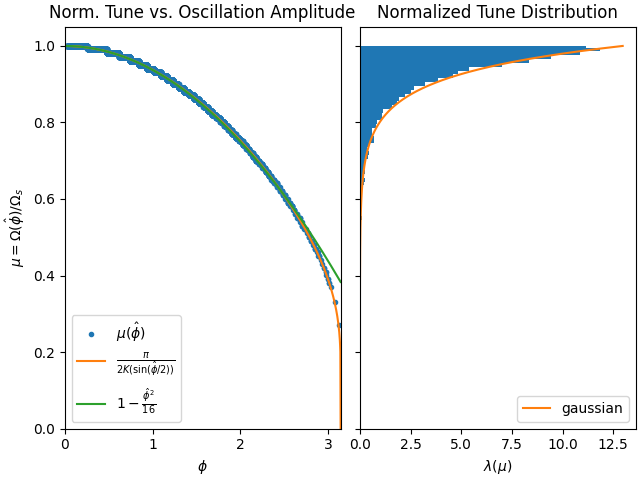
\includegraphics{figs/single_particle_motion/normalized_tune.png}
    \caption{Spread of synchrotron tune with oscillation amplitude}
    \label{fig:tune_spread}
\end{figure}

\section{Longitudinal Space Charge}

\subsection{Wakefields}

Consider a particle trailing behind other particles within a bunch. This particle will experience a voltage change due to the wake field of the preceding particles. A particle's induced voltage is given by the convolution of the linear charge density $\lambda(\tau)$ and this wake function $\mathcal{W}(\tau)$ \cite{wiedemann_particle_2015}\cite{zotter_impedances_1998}.

$$\Delta V(\tau)=-\int_0^\infty\lambda(t)\mathcal{W}(\tau-t)dt=-\mathcal{W}*\lambda$$

Where a bunch's longitudinal charge profile $\lambda(\tau)$ is normalized to the total charge $Q$:

$$Q = \int_{-\infty}^\infty \lambda(\tau) d\tau$$

We can define the impedance $Z(f)$ and spectrum $S(f)$ from the Fourier transforms of the wake function $\mathcal{W}(\tau)$ and charge profile $\lambda(\tau)$ respectively:

$$\begin{aligned}
        Z(f) & =\int_{-\infty}^\infty\mathcal{W}(\tau)e^{-i\omega\tau}d\tau \\
        S(f) & =\int_{-\infty}^\infty\lambda(\tau)e^{-i\omega\tau}d\tau
    \end{aligned}$$

The convolution of the wake function and linear charge density can be written as the inverse Fourier transform of the product of the spectrum and the impedance, therefore the induced voltage can be re-written as:

$$\Delta V(\tau)=-\int_{-\infty}^\infty S(f)Z(f)e^{i\omega \tau}df$$

For a linear impedance source such that $Z/n$ is constant where $n = f/f_s$, the impedance term can be separated from the integral so that the inverse Fourier transform of the spectrum can be incorporated instead as the derivative of the linear charge density:

\begin{equation}
    \Delta V=\frac{-i}{\omega_s}\frac{Z}{n}\frac{d\lambda}{d\tau}
    \label{eq:induced_voltage}
\end{equation}

\subsection{Space Charge Impedance}

The relativistic longitudinal self fields of a particle in a slowly varying coasting beam can be defined by the following\cite{ferrario_space_2014}:

$$E_z=-\frac{\bar{g}}{2\pi\epsilon_0\gamma^2}\frac{\partial \lambda}{\partial z}$$

Where the \textit{geometry factor} $\bar{g}$ is defined by (\ref{eq:longitudinal_self_fields}):

$$\bar{g}=\int_r^b\frac{f(r')}{r'}dr'\qquad f(r)=\frac{\int_0^r\rho(r')r'dr'}{\int_0^\infty\rho(r')r'dr'}=\frac{Q'}{Q}$$

Where Q' defines the amount of charge enclosed within the radius $r$. About a turn, these self fields will induce a voltage that can be defined as the \textit{Longitudinal Space-Charge Impedance}, given by \cite{lee_accelerator_2004}:

\begin{equation}
    \frac{Z}{n} = -i\frac{Z_0}{\beta\gamma^2}\bar{g}
    \label{eq:space_charge_impedance}
\end{equation}

The space-charge impedance can therefore be used to characterize the effective voltage drop of particles within a bunch by combing Equations \ref{eq:induced_voltage} and  \ref{eq:space_charge_impedance} to yield our induced space-charge voltage $\Delta V_{SC}$ as a function of the derivative of linear charge density profile and the geometry factor.

$$\Delta V_{SC} = -\frac{d\lambda}{d\tau}\frac{Z_0}{\beta_s\gamma_s^2}\frac{\bar{g}}{\omega_s}$$

The geometry factors as a function of transverse radial position $\bar{g}(r)$ for a uniform (\ref{eq:g_uniform}), parabolic (\ref{eq:g_parabolic}) and gaussian (\ref{eq:g_gaussian}) are depicted in Figure \ref{fig:geometry_factors}.

\begin{figure}
    \centering
    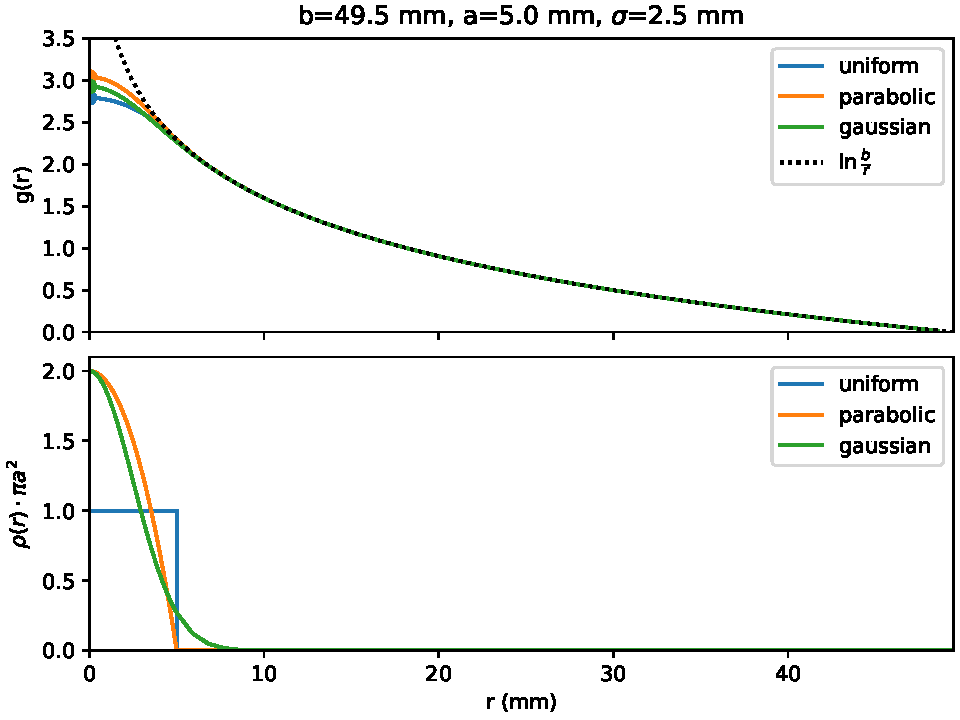
\includegraphics{./figs/geometric_factors.pdf}
    \caption{Geometric for varying radial charge profiles}
    \label{fig:geometry_factors}
\end{figure}

We observe that these various geometric factors used to represent the self fields of particles in or outside equivalently sized uniform, parabolic or gaussian round beams are mostly equivalent. 

The geometry factor for an particle ($r=0$) in a uniform circular bunch of radius $a$ in conducting aperture $b$ is given by:

$$\bar{g} = \frac{1}{2} + \ln\frac{b}{a} - \frac{1}2{}\frac{r^2}{a^2}$$

The maximum geometry factor, ($g(r=0)$) corresponding to maximum space-charge effects. Particles with large dispersion ($\delta$) or transverse emittance ()$\epsilon_\perp$) will pursue misaligned betatron trajectories with non-zero effective radial position, and therefore will incur reduce space-charge effects.

\subsection{Tune Shift}

Relevant to the oscillation frequency, it is also worth defining the space-charge impedance voltage gradient:

\begin{equation}
    V'_{SC}(\tau) = \frac{Z_0}{\beta\gamma^2}\frac{\bar{g}}{\omega_s}\frac{d^2\lambda}{d\tau^2}
\end{equation}

The normalized tune shift due to space-charge impedance can be defined by:
\begin{equation}
    \mu^2 = \frac{\Omega^2}{\Omega_s^2} = 1 + \frac{V'_{SC}}{V'_{RF}} = 1 + \frac{Z_0}{\beta\gamma^2}\frac{\bar{g}}{\omega_s}\frac{d^2\lambda}{d\tau^2}
    \label{eq:tune_shift}
\end{equation}

Consider a parabolic charge distribution defined between $\tau = \pm L_\tau/2$:

$$\lambda(\tau)=\frac{3Q}{2L_\tau}\left(1-4\frac{\tau^2}{L_\tau^2}\right)$$

The linear charge density is therefore defined by:

$$\frac{d\lambda}{d\tau} = \frac{-12Q}{L_\tau^3}\tau$$

The induced voltage gradient of a parabolic bunch due to space charge is given by Equation \ref{eq:vp_sc} \cite{lasheen_longitudinal_2016}. Because synchrotron frequency is proportional to the square of the voltage gradient, the effect of space-charge impedance is a frequency offset or shift such that $\Omega^2 \propto V'_{RF} + V'_{SC}$.

\begin{equation}
    V'_{SC} = -\frac{12Q}{\omega_s}\frac{\Im (Z)}{n}\frac{1}{L_\tau^3}=-\frac{12Q}{\omega_s}\frac{Z_0}{\beta_s\gamma_s^2}\frac{\bar{g}}{L_\tau^3}
    \label{eq:vp_sc}
\end{equation}

The effects of space-charge impedance to cause a synchrotron frequency shift can be observed in the tune distributions seen in Figure \ref{fig:tune_shift}.

\begin{figure}
    \centering
    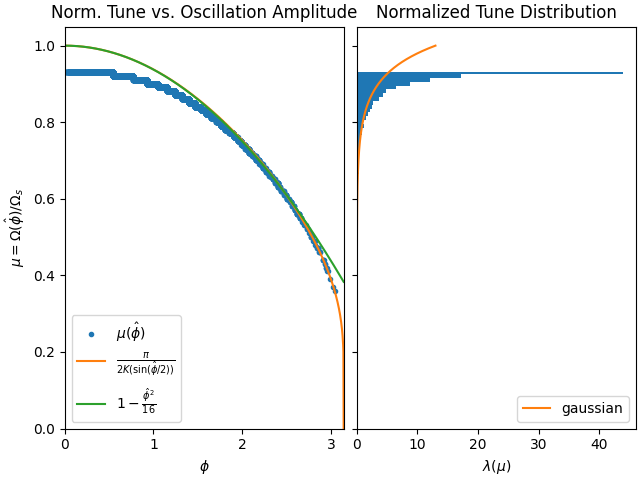
\includegraphics{figs/tune_shift/normalized_tune.png}
    \caption{Space-charge tune shift for 30 ns bunch, 2.08e12 protons, bunch}
    \label{fig:tune_shift}
\end{figure}

Here we have assumed a uniform space-charge geometry factor which fails to account for betatron motion variation and the non-uniform nature of the quasi-elliptical PS aperture.

\chapter{Aperture Reconstruction}

\section{Introduction}

As discussed in the previous chapter, the effects of longitudinal space-charge impedance is described in part by a characteristic geometry factor, describing the induced longitudinal fields due to the position a particle occupies within a transverse bunch distribution in a finite conducting aperture. To re-iterate, the geometry factor describing the longitudinal fields felt of a particle within a uniform circular bunch can be described by:

$$\bar{g}(r) = \frac{1}{2} + \ln\frac{b}{a}-\frac{1}{2}\frac{r^2}{a^2}$$

Much of this work revolves on accurately tracking and characterizing the beam size ($a$) and particle radius ($r$) relevant to this equation, however the PS's model for beam pipe aperture ($b$) is of unknown precision and many years out of date, to wit the updating of said aperture profile by manual tallying is time consuming, tedious, and error prone.

\begin{figure}
    \centering
    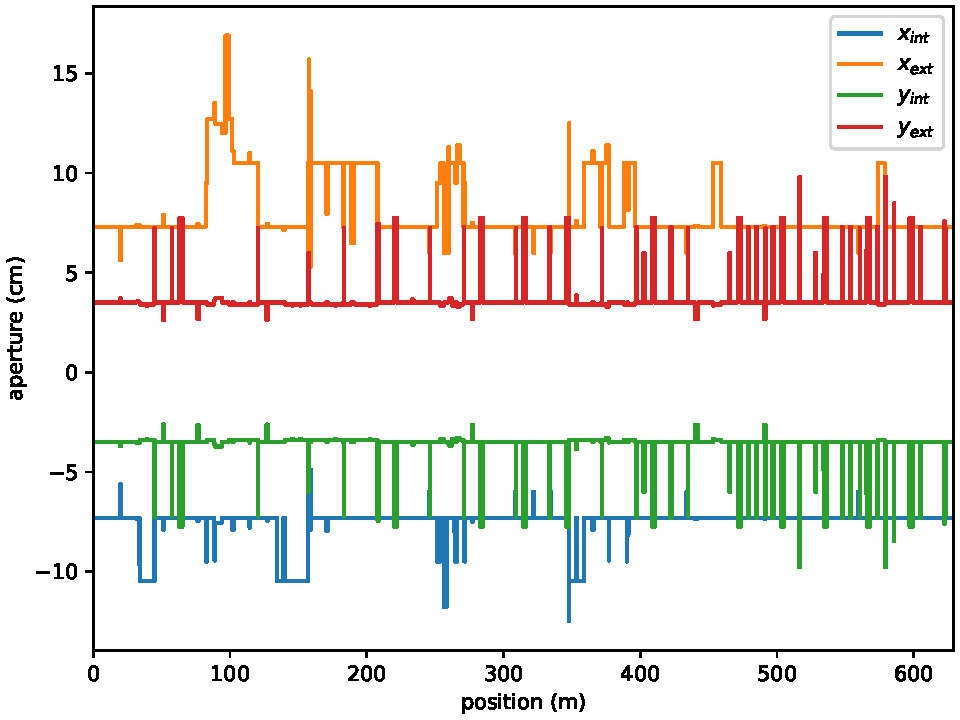
\includegraphics{figs/ps_aperture.pdf}
    \caption{Model of PS Aperture from 2013}
    \label{fig:ps_aperture_model}
\end{figure}

The most recent model, as depicted in Figure \ref{fig:ps_aperture_model}, is old and assumes for elliptical geometries. Though this is mostly valid for most of the ring, being an elliptical beam pipe of 35 x 73 mm wide, there are numerous nuanced cross sections of varying components such as septa, bellows, pump-out ports, etc. whose electrical boundaries aren't incorporated into this model.

\section{Intersection Algorithm}

The PS and it's sub-assemblies can be conveniently represented as triangular meshes, portable in STL (stereo-lithography) files, as depicted in Figure \ref{fig:ps_mu}.

\begin{figure}
    \centering
    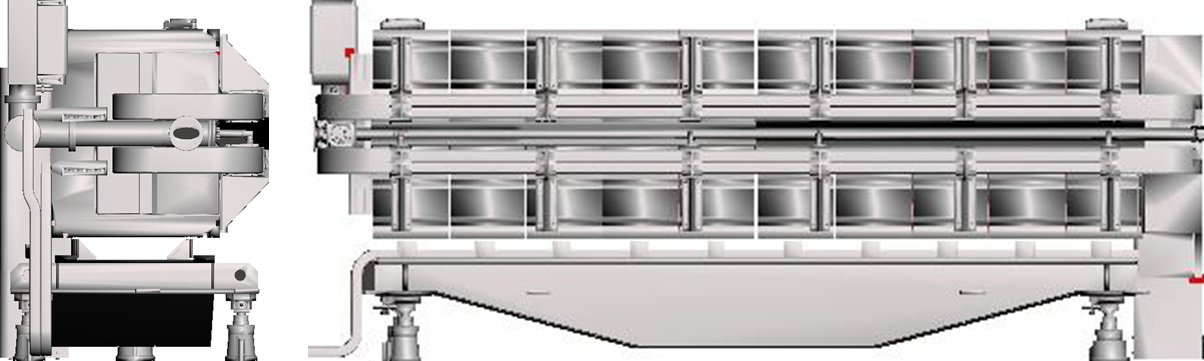
\includegraphics{figs/ps_magnet.png}
    \caption{Triangular mesh representation of a PS Dipole Magnet Unit (MU)}
    \label{fig:ps_mu}
\end{figure}

The objective is to define a reference-trajectory $R(\phi)$ in curvilinear coordinates consistent with a ``Frenet-Serret" coordinate system ($r,\theta,\phi$) such that a torus can be ``inflated" until collision with the electrical aperture of the model. 

Our toroidal coordinates are given by:

$$\begin{aligned}
        x & = (R(\phi)+r\cos\theta)\cos\phi \\
        y & = (R(\phi)+r\cos\theta)\sin\phi \\
        z & = r\sin\theta
    \end{aligned}$$

Where $R(\phi)$ serves the reference radius is is defined by the geometry of the PS's 100 straight sections (SS) and 100 magnet units (MU). A schematic of the reference trajectory for one of the PS's 36$^\circ$ sub-sectors is depicted in Figure \ref{fig:ref_traj}.

\begin{figure}
    \centering
    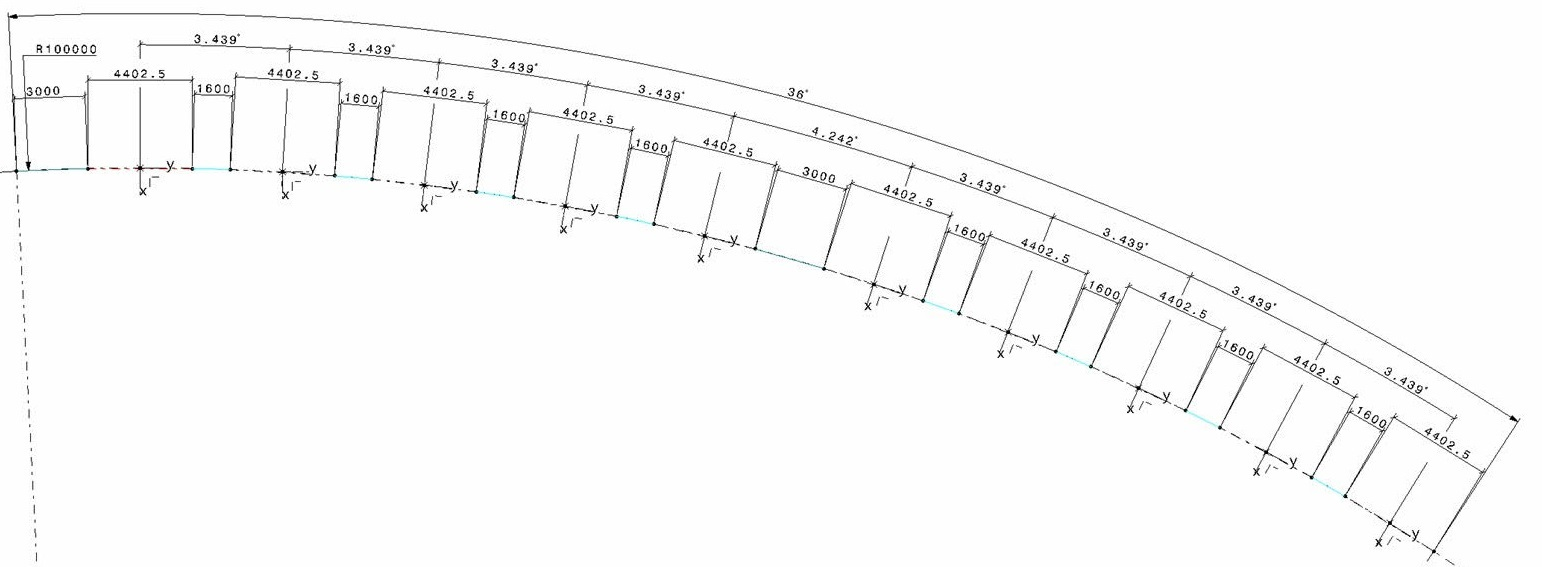
\includegraphics{figs/reference_trajectory_path.jpg}
    \caption{Engineering drawing of reference trajectory in a PS sector}
    \label{fig:ref_traj}
\end{figure}

We can use this definition of reference trajectory $R(\phi)$ to ``unwrap" the PS ring model into equivalent linear components as if the PS was a Linear accelerator, transforming our model coordinates into curvilinear $(x, y, s)$ and so to detect the aperture, a straight cylinder originating about the reference trajectory needs to be "inflated" until an intersection between surfaces is detected and recorded.

\section{Moller-Trumbore}

To perform this virtual "inflation" of our collision surface with our mechanical model, the \textit{Möller–Trumbore}\cite{moller_fast_1997} intersection algorithm can be used to compute intersection angles with the PS. It is commonly used in 3D graphics to efficiently detect and compute the intersection between light rays and polygons as well is it easily parallelized. In Figure  \ref{fig:ray_casting}, a point source is cast through a spherical shell to demonstrate the technique. The algorithm is able to evaluate each light ray with all faces to determine if an intersection is possible and if so, where.

\begin{figure}
    \centering
    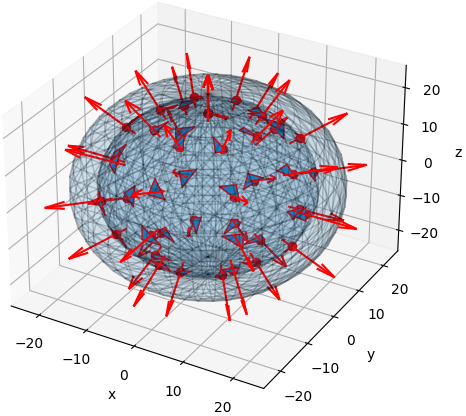
\includegraphics{figs/ray_casting.png}
    \caption{Rays cast from a point source through a spherical shell}
    \label{fig:ray_casting}
\end{figure}

After transforming the cartesian mechanical model of the PS to curvilinear coordinates, a line source was ``illuminated" along the central beam path whose ray intersections where detected. The was performed on each of the 100 magnet units and straight sections individually and then combined to produced an updated and detailed aperture as depicted in \ref{fig:ps_aperture}. The distinctive colors of the newly defined aperture coincide with a preservation for component granularity, being able to attribute specific aperture coordinates along the beam path with a particular magnet unit or straight section, allowing for easy verification.

\begin{figure}
    \centering
    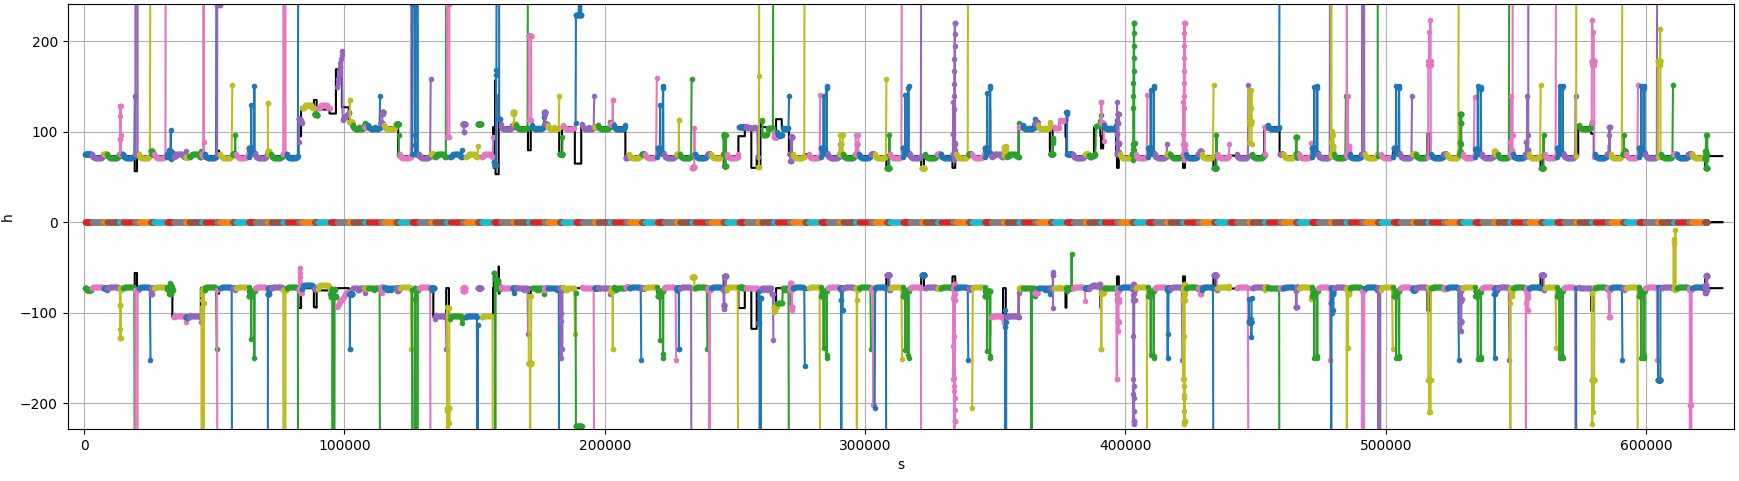
\includegraphics[width=\linewidth]{figs/ps_aperture.png}
    \caption{Horizontal aperture of the PS reconstructed by Ray Casting}
    \label{fig:ps_aperture}
\end{figure}

By using this automated technique as opposed to a manual aperture accounting, details could be queried at much higher longitudinal and poloidal resolutions, as seen in Figure \ref{fig:ps_aperture_hi_res}. Additionally, features for smaller and yet frequent discrepancies could be automatically identified as in the case of pump-out ports and bellows.

\begin{figure}
    \centering
    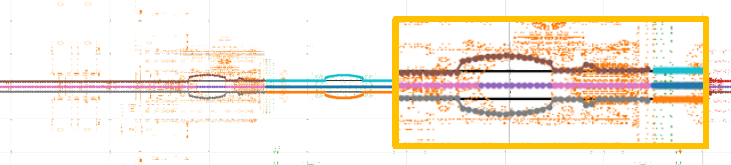
\includegraphics{figs/apertture_hi_res.PNG}
    \caption{Hi-Res reconstruction of PS aperture}
    \label{fig:ps_aperture_hi_res}
\end{figure}

Additionally, details of RF cavities, diagnostic ports and septa can be compared with that of the older model per Figure \ref{fig:ps_septa}.

\begin{figure}
    \centering
    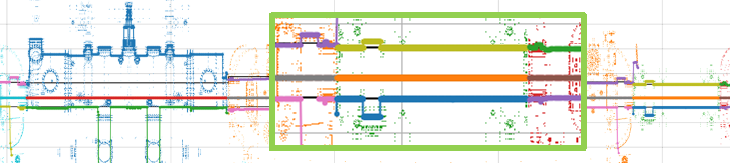
\includegraphics{figs/aperture_comparison.PNG}
    \caption{Comparison of updated aperture model with 2013 version (Black)}
    \label{fig:ps_septa}
\end{figure}

\chapter{Simulation}

\section{Transverse Tracking}

The optics of the PS are described by the beta function ($\beta(s)$) and dispersion function ($D(s)$) as depicted in Figure \ref{fig:ps_optics}.

\begin{figure}
    \centering
    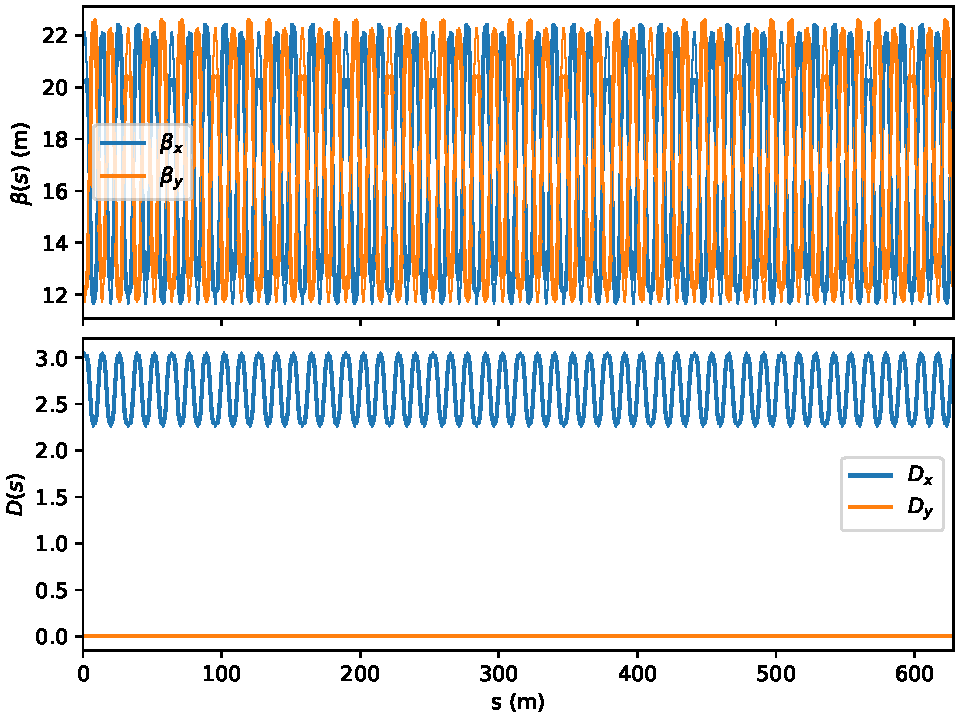
\includegraphics{figs/ps_optics.pdf}
    \caption{Transverse optics of the PS}
    \label{fig:ps_optics}
\end{figure}

For simplicity of transverse tracking purposes and subsequent development of analytic relationships, the periodicity of these optics can be accurately represented as a two-term Fourier series:

\begin{equation}
    \beta(\theta) \approx \sum_k \beta_k e^{i k\theta} \qquad D(\theta) \approx \sum_k D_k e^{i k\theta}
    \label{eq:optics_decomposition}
\end{equation}

The coefficients describing the PS optics to first order are described in Table \ref{tab:ps_optics_fourier} as consistent with Equations \ref{eq:optics_decomposition}. This approximation helped in reducing the computation time for the subsequent transverse tracking simulations and avoiding interpolation artifacts.

\begin{table}
    \centering
    \begin{tabular}{c | c  r | c  r }
        $\beta_x(\theta)$ & $\beta_{0,x}$ & 16.89 & $\beta_{50,x}$ & +4.43-2.84i \\
        $\beta_y(\theta)$ & $\beta_{0,y}$ & 17.01 & $\beta_{50,y}$ & -4.46+2.86i \\
        $D_x(\theta)$     & $D_{0,x}$     & 2.66  & $D_{50,x}$     & +0.34-0.22i \\
        $D_y(\theta)$     & $D_{0,y}$     & 0     & $D_{50,y}$     & 0           \\
    \end{tabular}
    \caption{Primary Fourier coefficients describing periodic nature of PS optics}
    \label{tab:ps_optics_fourier}
\end{table}

A transverse tracker was developed to solve for betatron trajectories described by solutions to Hill's Equations (Equations  \ref{eq:hills_equations}). A bivariate gaussian distribution with matching covariance matrix ($\Sigma$) to that of the PS's Twiss matrix ($\Omega$) was ``injected" and tracked about one turn in the synchrotron as depicted in Figure \ref{fig:trans_tracking}.

\begin{figure}
    \centering
    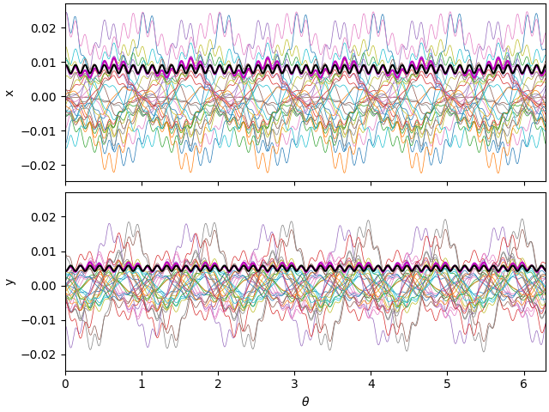
\includegraphics{figs/transverse_tracking.png}
    \caption{Faded trajectories of select particles alongside statistical (magenta) and analytic (black) beam widths in the PS}
    \label{fig:trans_tracking}
\end{figure}

\subsection{Effective Geometry Factor}

Given the ability to track the transverse locations of individual particles propagating through the PS lattice relative to the transverse particle distribution itself, each particle's geometry factor can be computed and observed to vary along the ring. These geometry factors can be averaged resulting in the definition of the effective geometry factor, characterizing the particle's turn-averaged experienced space-charge, dependent on the optics, aperture, and the particle's characteristic emittance, phase advance and dispersion.

$$g_{EFF} \propto g(\epsilon_\perp, \mu_0, \delta)$$

The transverse tracker was accordingly used to build a response matrix to predict a particle's effective geometry factor given it's initial conditions ($\epsilon_x, \epsilon_y, \delta$) within a known beam of characteristic statistics ($\epsilon_\perp, \sigma_\delta$). In relation to dispersion, Figure \ref{fig:g_eff_dispersion} indicates a parabolic dependence with the effective geometry factor and a linear relationship with transverse emittance. A particle's phase-advance appears to have minimal impact on the effective geometry factor.

$$g_{eff} \propto g_{max} - C_0\delta^2 - C_1\epsilon_x - C_2\epsilon_y$$

\begin{figure}
    \centering
    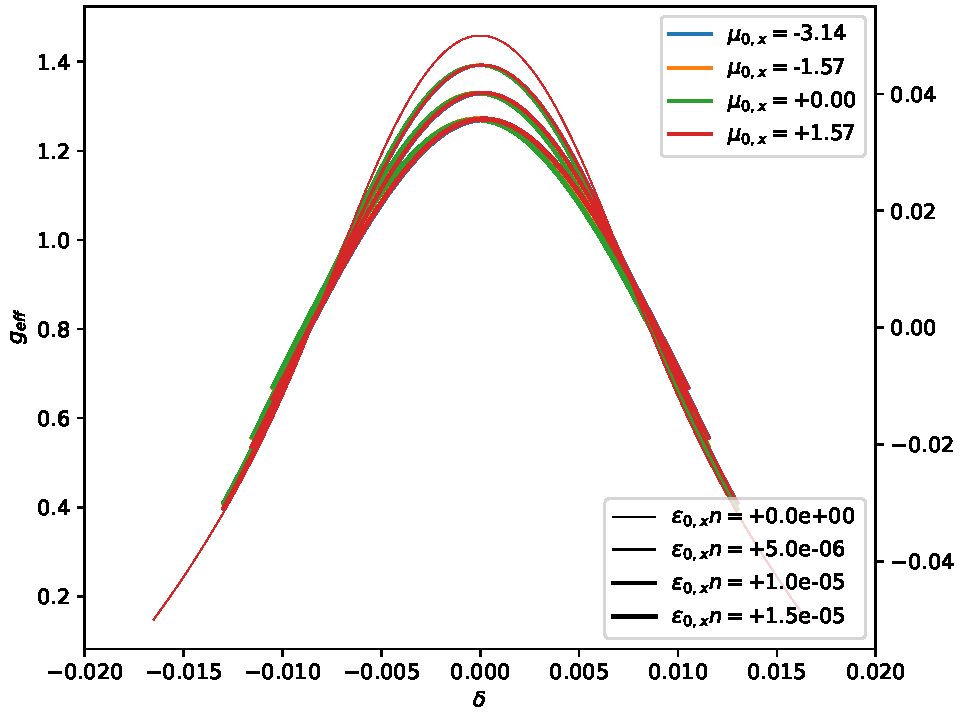
\includegraphics{figs/g_dispersion.pdf}
    \caption{Impact of particle \textbf{dispersion} on effective geometry factor}
    \label{fig:g_eff_dispersion}
\end{figure}

We see however that the domain for $g_{eff}$ is limited as particles with a combination of very high dispersion or very high emittance are likely to collide with the beam aperture and are counted as lost particles. This phenomena is more readily visible in Figure \ref{fig:g_emittance} where we see the thicker lines (representing higher dispersion) end up being truncated with increased transverse emittance. This figure also makes it more clear the exponential relationship between emittance and the geometric factor when dispersion is low.

\begin{figure}
    \centering
    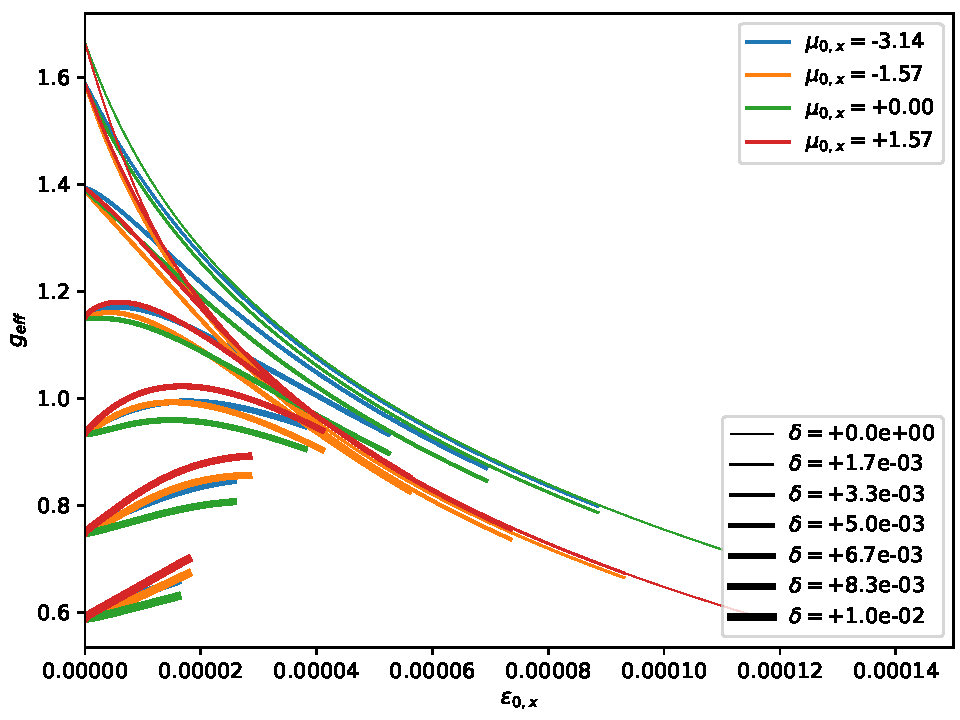
\includegraphics{figs/g_emittance.pdf}
    \caption{Impact of particle \textbf{emittance} on effective geometry factor}
    \label{fig:g_emittance}
\end{figure}

We see in Figure \ref{fig:g_phase_advance} that though changes in geometry factor are dominated by dispersion and particle emittance, along the course of a particle around it's elliptical trajectory in transverse phase-space, there will be a quasi-sinusoidal impact on the geometry factor due to phase-advance, though this can largely be neglected.

\begin{figure}
    \centering
    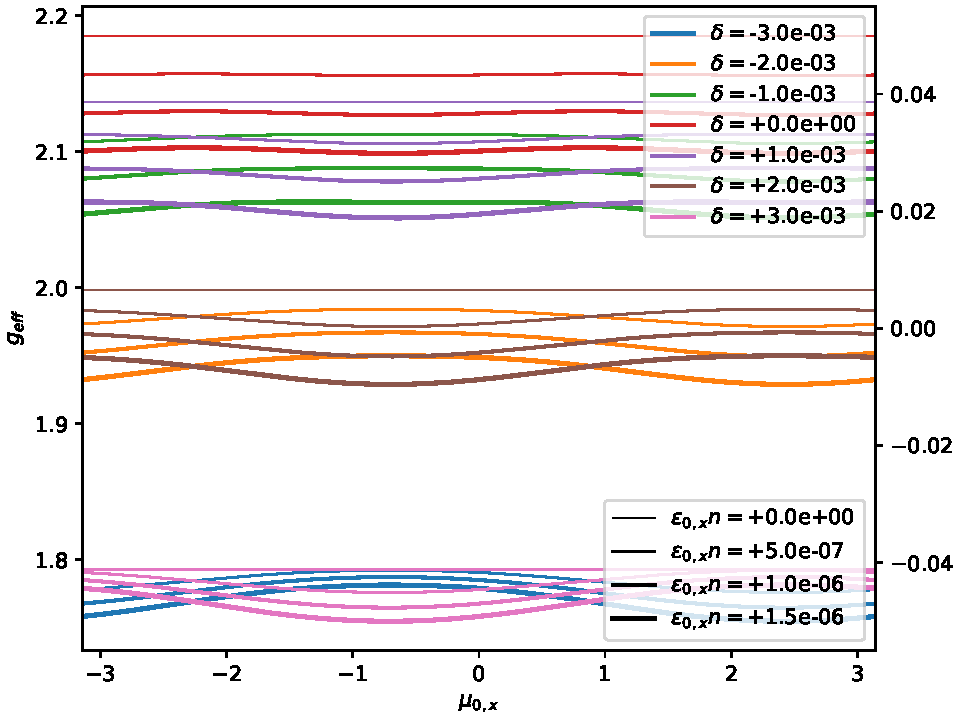
\includegraphics{figs/g_phase_advance.pdf}
    \caption{Impact of particle \textbf{phase advance} on effective geometry factor}
    \label{fig:g_phase_advance}
\end{figure}

This complicated relationship can be summarized in a lookup table or response matrix as visualized in Figure \ref{fig:g_eff_vol}.

\begin{figure}
    \centering
    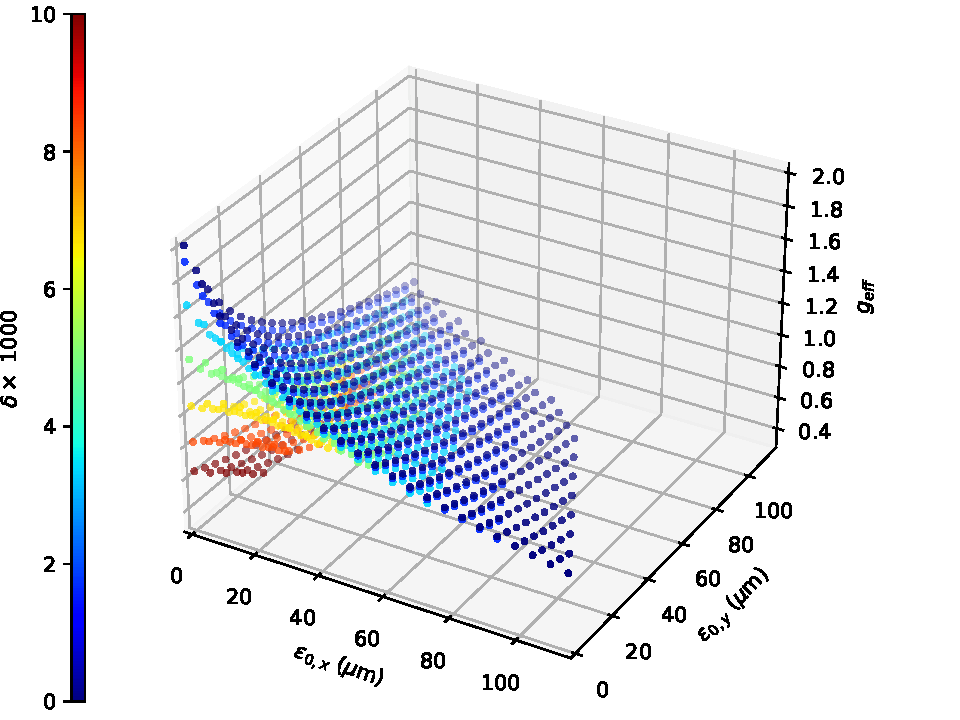
\includegraphics{figs/g_eff.surface.0.pdf}
    \caption{Multi-dimensional vector space of effective geometry factor}
    \label{fig:g_eff_vol}
\end{figure}

The impact of particle phase-advance was neglected as it's effect is minimal in comparison to the other dependencies on account of the fact that the transverse tune is large and accordingly a variation in a particle's initial phase-offset will contribute to little variance in the particle's effective radial position.

\section{Longitudinal Tracking}

\subsection{Usage of Geometric Factor}

A longitudinal tracker can be developed by discretizing Equations \ref{eq:eom}, yielding the \textit{turn-by turn} ``kick" and ``drift" components respectively.

$$w_{i+1}-w_i \to \Delta w = qV(\tau) \qquad \tau_{i+1}-\tau_i \to \Delta\tau = \kappa T_s w$$

To include space-charge in our tracker, the induced voltage due to space-charge impedance is include with RF acceleration.

$$V(\tau) = V_{RF} + V_{SC}$$

Now $\bar{g}$ is replaced as found in Equation \ref{eq:space_charge_impedance} with the effective particle dependent geometry factor $g_{eff}$ for a parabolic longitudinal bunch given by:

$$V_{SC} = -\frac{12Q}{L_\tau^2}\frac{Z_0}{\beta\gamma^3}\frac{g_{eff}(\epsilon_x,\epsilon_y,\delta)}{\omega_s}$$

Transverse emittance $\epsilon_x$ and $\epsilon_y$ is presumed to be preserved between synchrotron ``kicks", however dispersion evolves with synchrotron motion and accordingly the geometry factor will notice an influence as the particle orbits in longitudinal phase-space.

\subsection{Tune ``Blur"}

Consider we sample our distribution from a 6D ellipsoidal distribution coordinated with gaussian transverse emittance ($\epsilon_\perp$), uniform phase advance and gaussian dispersion ($\sigma_\delta$) and bunch length ($\sigma_\tau$). Using this modified longitudinal tracker, the normalized tune distribution incorporating the effective geometry factor due to transverse motion is given by Figure \ref{fig:tune_blurr} where we observe a ``blurred'' tune spread distribution for the synchrotron frequency.

\begin{figure}
    \centering
    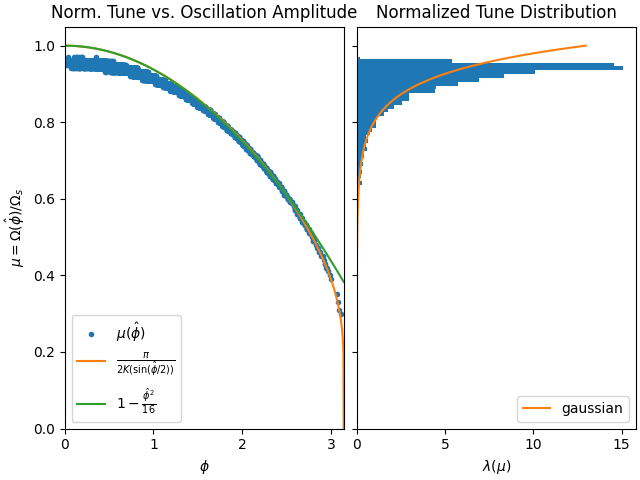
\includegraphics{figs/tune_blurr/blurred_tune.png}
    \caption{Blurred Synchrotron Frequency spread distribution due to space-charge impedance with transverse motion}
    \label{fig:tune_blurr}
\end{figure}

To improve tracking statistics and make more visible the phenomena, Figure \ref{fig:full_comparison} compares the three test cases of synchrotron motion.

\begin{figure}
    \centering
    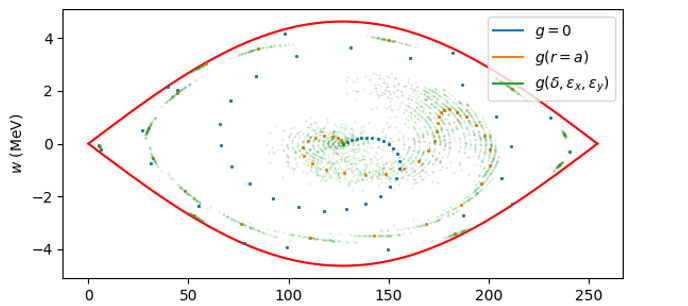
\includegraphics[width=\linewidth]{figs/tune_blurr/trajectories.png}
    \caption{Comparison of Synchrotron motion of ``ghost particles" in a matched longitudinal bunch for single-particle motion, coherent space-charge impedance and incoherent space-charge impedance incorporating betatron motion}
    \label{fig:full_comparison}
\end{figure}

The particles depicted are selected ``ghost" particles visualized within a non-oscillating matched longitudinal bunch. Accordingly, the derivative term related to the longitudinal profile is non-varying as the longitudinal profile is stable. Nonetheless we observe originally the deviation between single-particle motion ($g=0$), coherent space-charge impedance $g(r=a)$ and incoherent space-charge impedance $g(\delta, epsilon_x, \epsilon_y)$ which approximates betatron motion.

\begin{figure}
    \centering
    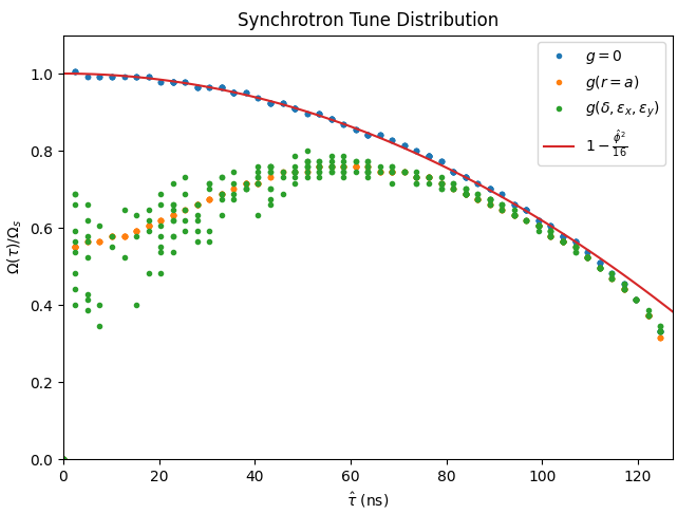
\includegraphics{figs/tune_blurr/normalized_tune.png}
    \caption{Blurring of synchrotron oscillation frequency due to Transverse Motion}
    \label{fig:tune_dist_blur}
\end{figure}

Furthermore, by incorporating an additionally nuanced transverse motion, we observe a "blurring" of the particles synchrotron frequency shift on account of the variance in particle's space-charge impedance. Though particles may occupy the same location in longitudinal phase-space, each particle's unique dispersion, emittance and phase-advance will modify it's respective kick differently and therefore it's revolution period along hamiltonian contours will vary as seen in Figure \ref{fig:tune_dist_blur}.

\subsection{Bunch Stability}

A standard \textit{dipole-oscillation} measurement to determine the synchrotron frequency is to observe the bunch length contraction frequency of a bunch injected with an longitudinal offset. Accordingly we can observe how an offset bunch will oscillate about the bucket center until it reaches a stable larger value where synchrotron motion has sufficiently filamented the mismatched distribution to that of a matched distribution with higher geometric emittance, as visible in Figure \ref{fig:filamentation}.

\begin{figure}
    \centering
    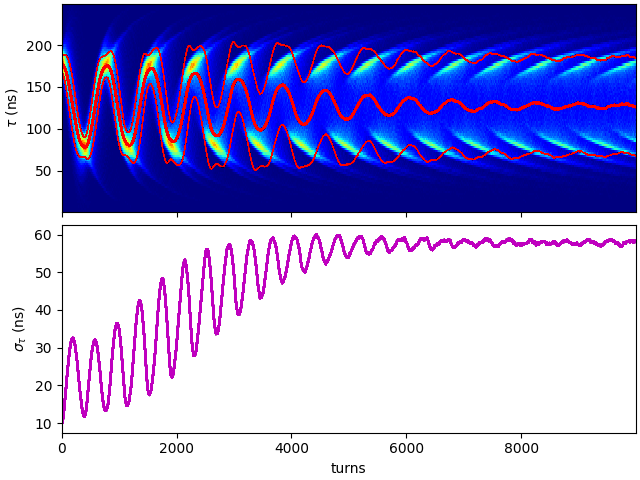
\includegraphics{figs/dipole_oscillation.png}
    \caption{\textbf{BLonD} simulation of dipole oscillations}
    \label{fig:filamentation}
\end{figure}

Tune blurring may increase the observed filamentation rate of our distribution. Filamentation, due to synchrotron frequency spread, is a fundamental phenomena in synchrotron motion. It is frequently associated as a stabilizing effect as mismatched bunches or coherent bunch perturbations will be eventually distributed along Hamiltonian contours until decoherence. Therefore, it is reasonable to suspect that the impact of transverse motion on longitudinal space-charge impedance may provide additional stability to longitudinal motion.

\chapter{Conclusions}

\section{PS Experiments}

And attempt to measure the phenomena of ``tune blurring" with experiments at \textit{Flat-Bottom} were conducted with the following baseline parameters for the PS:

\begin{table}
    \centering
    \begin{tabular}{c|c |c |c}
        parameter  & symbol     & value & unit      \\
        \hline
        harmonic   & h          & 9     &           \\
        voltage    & $V_g$      & 22    & kV        \\
        intensity  & N          & 2e12  & particles \\
        transition & $\gamma_t$ & 6.1   &           \\
    \end{tabular}
    \caption{PS parameters in \textbf{MD} experiments}
    % \label{tab:my_label}
\end{table}

Bunch length and instability measurements can be used to characterize and identify the synchrotron frequency \cite{sacherer_bunch_1977}. A unmatched but centered bunch will contract in accordance with the synchrotron frequency. This forms a \textit{quadrupole-oscillation} in bunch length which can be measured and interpreted to yield information for the distribution's synchrotron frequency.

\begin{figure}
    \centering
    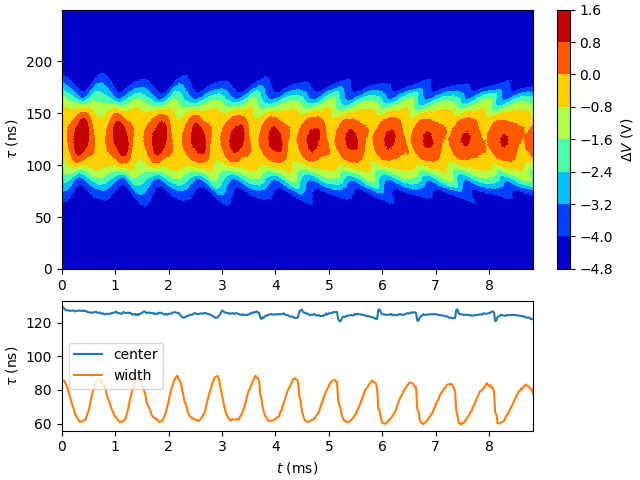
\includegraphics{figs/injosc.14x144.dat.npy.png}
    \caption{Bunch length oscillations from PS intensity experiments}
\end{figure}

In experiment, only the ``bulk" bunch length can be probed to derive information regarding the distributions synchrotron oscillation frequency however because synchrotron motion and space charge require a tune spread, offset and potentially a ``blur", resolving this information from the evolution of 1D longitudinal profiles is challenging.

The analysis of these measurements were inconclusive as intrinsic beam instabilities incorporated a high variance between similar measurements. As well, the beam become unstable at higher bunch intensities. It would still however be potentially fruitful to further conduct these measurements over a longer period of time so that the additional synchrotron oscillations measured may provide sufficient detail to quantify the effect of transverse motion on filamentation rate.

\section{Summary}

It has been shown in theory and simulation that the unique motion of a particle's betatron trajectories will provide additional variance to the applied induced voltage due to space-charge impedance. This effect, when capture adequately in longitudinal tracking codes, yields an observed "blurring" of the synchrotron frequency distribution when compared to that of less sophisticated approaches. The observed tune blur leads to an increased filamentation rate and accordingly may suggest an increase to the dampening rate longitudinal fluctuations and micro-bunch instabilities. Attempts to measure this filamentation rate variation were unsuccessful however further work may be conducted over a sufficiently long acquisition period so that an oscillating bunch can be observed to fully stabilize to provide further insight to the filamentation rate.